\documentclass{css}
%\documentclass[english]{css}

\usepackage[dvips]{graphicx}
\usepackage{latexsym}

\def\|{\verb|}

\newcommand{\cssyear}[0]{2023}
\newcommand{\cssname}[0]{CSS 2023}
\newcommand{\cssversion}[0]{2023/06/01}
\newcommand{\cssemail}[0]{css2023-office@iwsec.org}

\begin{document}

%% 本文が和文の場合,タイトル・著者名・著者所属・概要は,和文・英文共に必須.
%% If you prepare this manuscript in English, there is no need to put Japanese metadata (title, author names, affiliations, abstract, and keywords) in it.

\title{Isolation Forestを用いた\\IoT向け異常検知手法に関する考察}
\etitle{A Study on Anomaly Detection Method \\for IoT using Isolation Forest}

\affiliate{XX}{東京工業大学 情報理工学院 数理・計算科学系\\
Department of Mathematical and Computing Sciences, School of Computing, Tokyo Institute of Technology}
\affiliate{YY}{株式会社YYセキュリティ研究所\\
Security Laboratories, YY Corporation}
\paffiliate{ZZ}{国立研究開発法人ZZ研究所\\
National Institute of ZZ}

%% メールアドレスは省略可能だが,代表者のメールアドレスは必須.
%% 姓名の間は半角スペースを入れること.

\author{菅田 大輔}{Daisuke Sugata}{XX}[sugata.d.aa@m.titech.ac.jp]
\author{安全 花子}{Hanako Anzen}{XX, YY, ZZ}

%% the following is author command for english option.
%% at least one e-mail address is required.

%\author{Taro Joho}{XX}[taro.joho@xx.ac.jp]
%\author{Hanako Anzen}{XX, YY, ZZ}

\begin{abstract}
概要

\end{abstract}

%% キーワード (1--5単語) の記載は任意.

\begin{jkeyword}
Isolation Forest, IoT, IDS, 異常検知
\end{jkeyword}

\begin{eabstract}
abstract

\end{eabstract}

%% the following keyword part is optional and can be omitted.

\begin{ekeyword}
Isolation Forest, IoT, IDS, Anomaly Detection
\end{ekeyword}

%% if you use english opsion, you should put your English abstract in the abstract environment.
%% eabstract is not displayed in english mode.

\maketitle

%1
\section{はじめに}
以下のことを書く.

\begin{itemize}
    \item 大目標:小規模な環境向けのIoT向け異常検知手法の提案・「IoT環境を考えたとき、iforestが軽量でうまくいきそうなので、〜うまくいかないことも多かった。そこで、データセットの〜を工夫して、そのやり方を報告する」→本研究の目的を最初に述べちゃう
    \item 大目標を実現する必要性:卒論と同じ
    \item 問題提起(大目標を達成するために必要なことを述べ,そのためにどのような問題があるのかを述べる(小目標に分割する).)関連研究をリサーチしてみると参考にした論文が良さそうだ。しかし、いくつか課題もあるので改善したい
    1. 特徴量エンジニアリング 2. 判定の組み合わせアルゴリズム 
    \item (関連研究:問題を解決するための従来研究を紹介)
    \item 本研究の目的:1. 特徴量エンジニアリングの比較 2. 判定の組み合わせアルゴリズムの改善
\end{itemize}




\section{研究方法}

\subsection{Isolation Forestの説明}
Isolation Forest(以下,iForest)は,外れ値検出のためのアルゴリズムである。iForestは異常データが少数であり、離れているという前提に基づいている。ランダムにデータを分割していくと、異常データは相対的に早く分離される。iForestは以下のステップで実行される。

\subsubsection*{1. データの分割}
ランダムに選んだ特徴量から、ランダムに選んだ値をもとにデータを分割する。これを一定回数繰り返し、複数のツリーを作成する。

\subsubsection*{2. 異常スコアの算出}
データがツリーの枝に到達するまでの平均パスをもとに、異常スコアを算出する。具体的な計算式は以下の通りである。

ここで、$E(h(x))$はデータ点$x$の平均パス長、$c(n)$はデータセットのサイズ$n$に依存する定数である。

\subsubsection*{3. 異常判定}
先ほど計算した異常スコアをもとに異常検知を行う。通常、トレーニングデータの異常スコアの上位10\%を閾値として設定し、それを超えたデータを異常と判定する。


\subsection{IDSの概要}

IDSの概要をかく.
採用した理由を述べる.

\subsubsection{全体像}
今回の研究では,以下のようなIDSで異常検知を行った.

\subsubsection{}


\section{事前実験}
Isolation Forestを異常検知手法として使用する際,どのような問題があるのかを明らかにするため,事前実験を行った.はじめにデモデータを使用して,iForestの挙動を確認した.その考察をもとに、特徴量選択手法の提案を行なった

使用したデモデータは、(2.5, 2.5)と(-2.5, -2.5)を中心とした
正常データ群と、10から-10の範囲に一様に分布した異常データ群からなる.二次元の場合のデモデータを図\ref{fig:demodata}に示す.

\begin{figure}[tb]
    \centering
    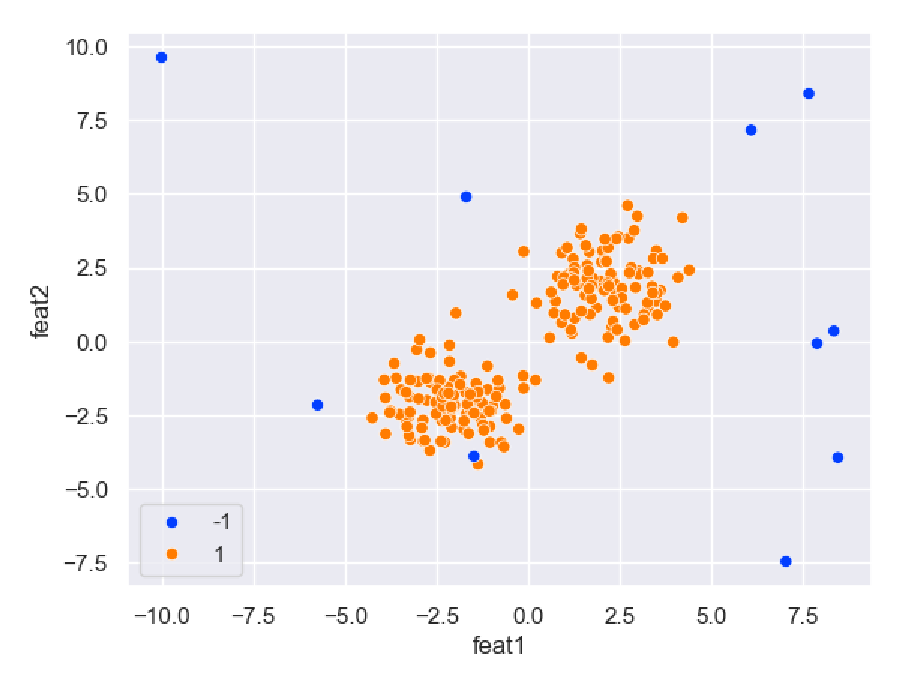
\includegraphics[width=\linewidth]{pictures/eps/demodata.eps}
    \caption{デモデータに関する図の説明(和文)}
    \ecaption{Description of the dim\_vs\_accu figure (English).}
    \label{fig:demodata}
\end{figure}

はじめに、デモデータと特徴量数の関係を調査した.図\ref{fig:dim_vs_accu}に示すように、特徴量数が増えるにつれて、異常検知の精度が単調に向上することがわかった.また、精度ののびは増加に比例して緩やかになっていることもわかる。ゆえに、iForestは十分な特徴量数が存在すると言える。

\begin{figure}[tb]
    \centering
    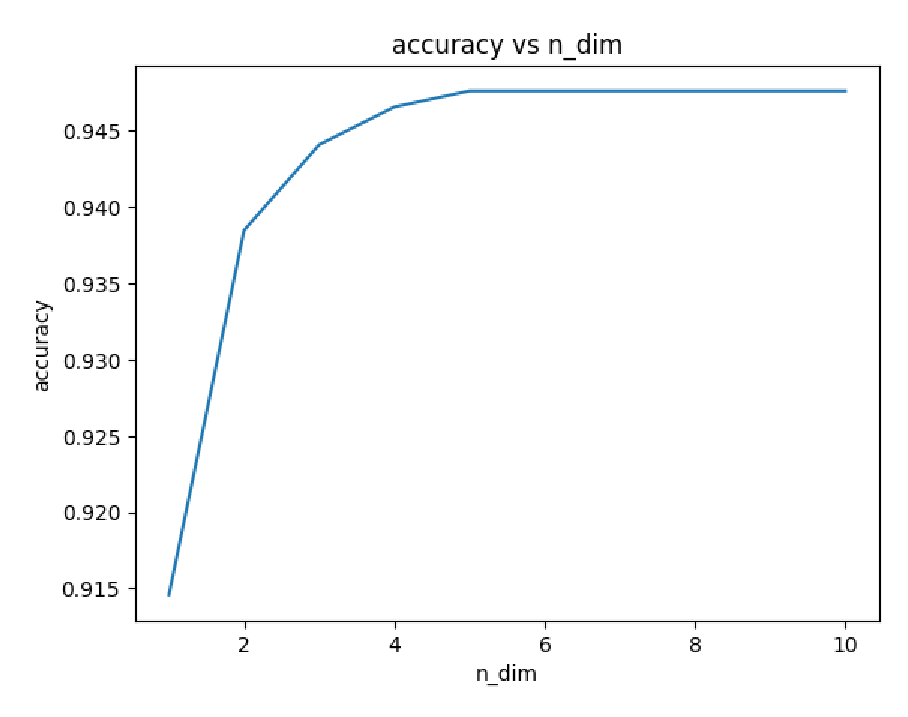
\includegraphics[width=\linewidth]{pictures/eps/dim_vs_accu.eps}
    \caption{dim\_vs\_accuに関する図の説明(和文)}
    \ecaption{Description of the dim\_vs\_accu figure (English).}
    \label{fig:dim_vs_accu}
\end{figure}

パケット通信を監視して得られたデータセットの全ての特徴が、異常検知に有効であるわけではない。iForestは特徴量同士の重みづけを行わないため、判定に有効でない特徴量が混ざると精度が低下すると考えられる。そこで、図\ref{fig:noise_accu}に示すように、ノイズとなる特徴量を混ぜた時の精度を調査した。この結果から、ノイズとなる特徴量が混ざると精度が低下することがわかった。また、今回の実験の場合だと、ノイズとなる特徴量が判定に有効な特徴量数の2倍以上になると、精度が急激に低下することがわかった。

\begin{figure}[tb]
    \centering
    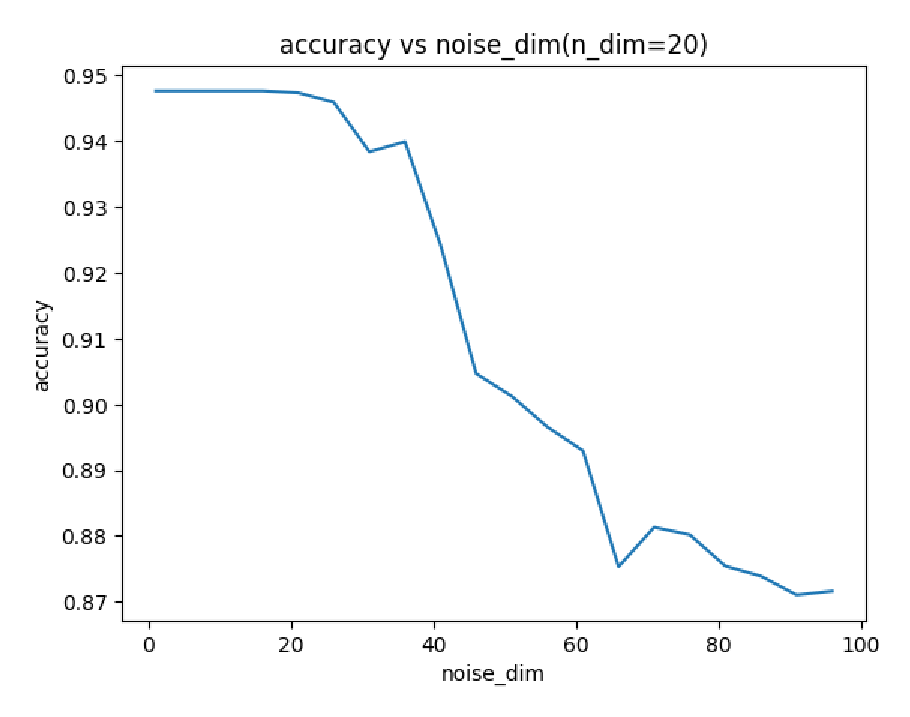
\includegraphics[width=\linewidth]{pictures/eps/noise_accu.eps}
    \caption{noise\_accuに関する図の説明(和文)}
    \ecaption{Description of the noise\_accu figure (English).}
    \label{fig:noise_accu}
\end{figure}

前の実験から、データセットからノイズとなる特徴量を取り除くことが重要であることがわかった。ところで、iForestはツリーベースの異常検知手法である。そこで、同じくツリーベースのRandam Forestから特徴の重要度を算出すれば、ノイズとなる特徴量を取り除けるのではないかと考えた。図\ref{fig:select_noise}は、Random Forestで算出した特徴量の重要度を表している。このグラフは、ノイズ特徴量を判別できていることがわかる。そして、実際にノイズ特徴量を取り除いた場合の精度を調査したところ、精度は???\%から0.945\%まで向上した。この結果から、Feature Importanceによる特徴量選択手法は精度の向上に有効ではないかと考えた。

\begin{figure}[tb]
    \centering
    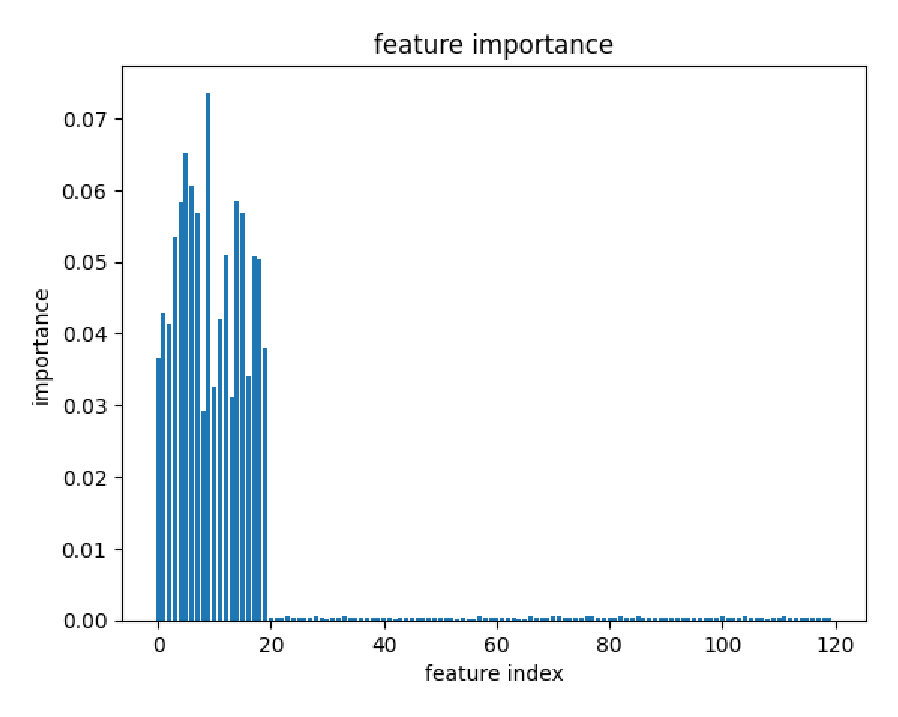
\includegraphics[width=\linewidth]{pictures/eps/select_noise.eps}
    \caption{select\_noiseに関する図の説明(和文)}
    \ecaption{Description of the select\_noise figure (English).}
    \label{fig:select_noise}
\end{figure}

\section{結果と考察}
(本論文のメイン)

\subsection{実験方法}

\subsubsection{実験環境}
他の人が再現できるように実験環境を書く.
1. 特徴量エンジニアリングの比較
2. 判定の組み合わせアルゴリズムの比較

\subsubsection{データセット}
使用したデータセットの概要と, その妥当性について述べる.

\subsubsection{評価指標}
使用した評価指標と, その妥当性について述べる.

\subsection{結果}
実験の結果,得られるデータから読み取れる客観的事実を書く.
この時, 論文の目的を達成するためにどのような主張をどのような結果(データ)に基づいて説明すべきかを考える.

\begin{figure}[tb]
    \centering
    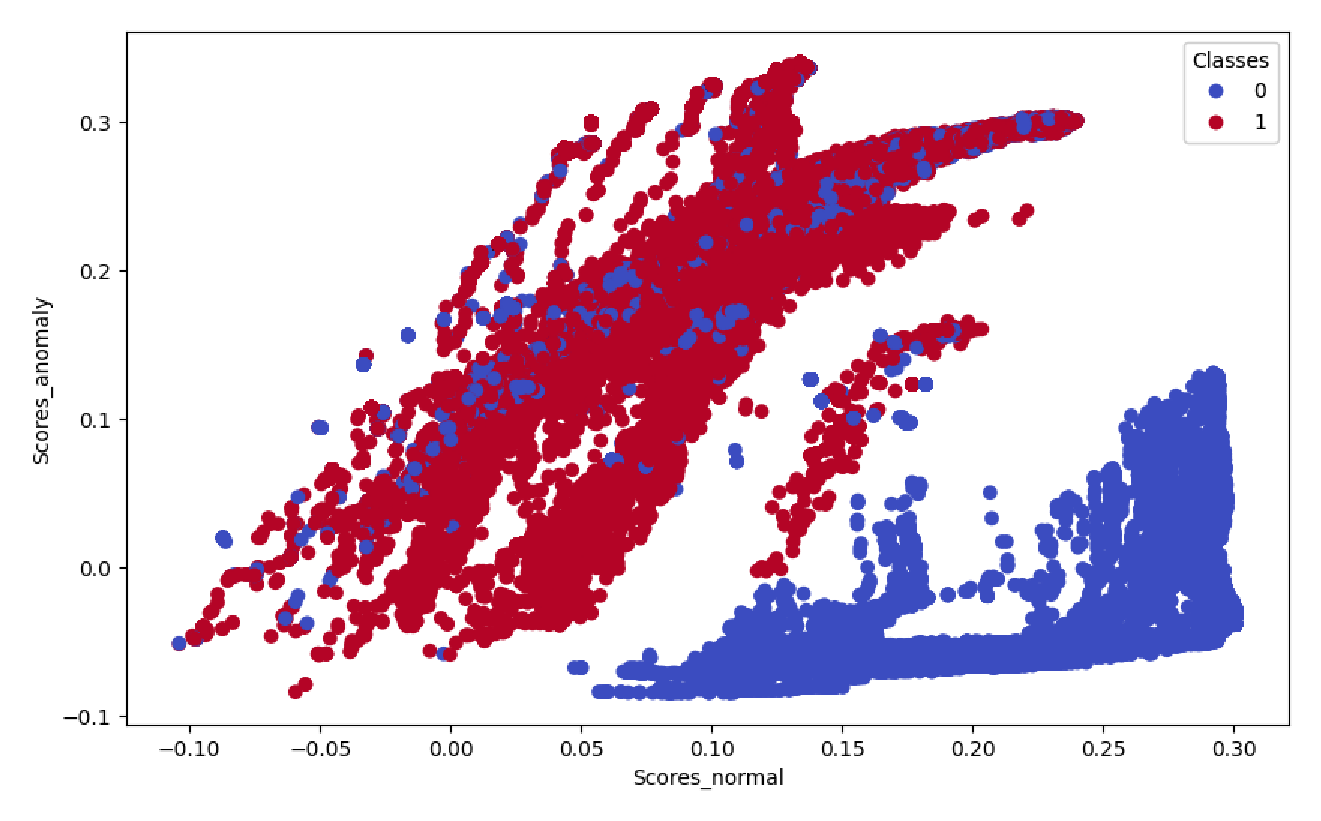
\includegraphics[width=\linewidth]{pictures/eps/classes_UNSW.eps}
    \caption{FI\_UNSWに関する図の説明(和文)}
    \ecaption{Description of the FI\_UNSW figure (English).}
    \label{fig:FI_UNSW}
\end{figure}

\begin{figure}[tb]
    \centering
    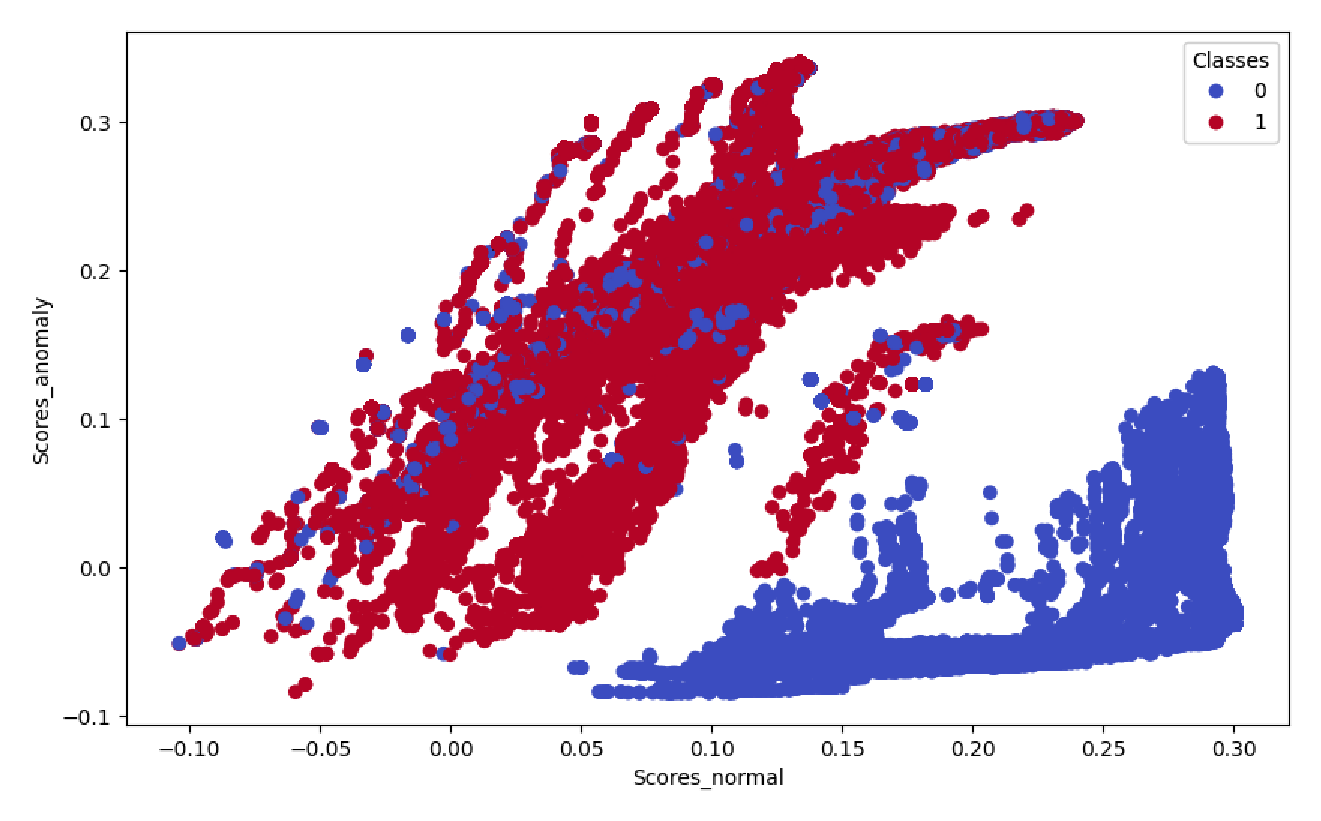
\includegraphics[width=\linewidth]{pictures/eps/classes_UNSW.eps}
    \caption{classes\_UNSWに関する図の説明(和文)}
    \ecaption{Description of the classes\_UNSW figure (English).}
    \label{fig:classes_UNSW}
\end{figure}

\begin{figure}[tb]
    \centering
    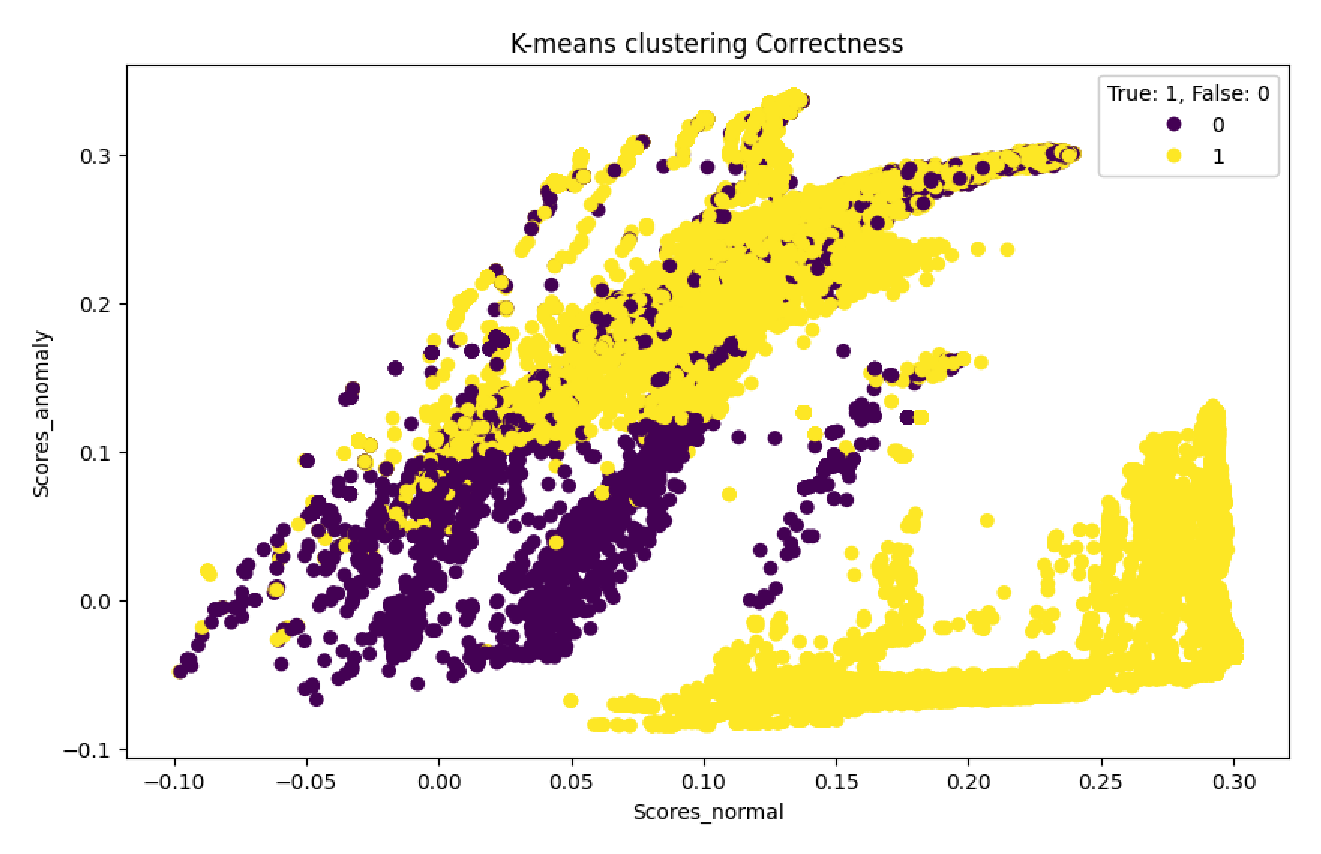
\includegraphics[width=\linewidth]{pictures/eps/collectness_UNSW.eps}
    \caption{collectness\_UNSWに関する図の説明(和文)}
    \ecaption{Description of the collectness\_UNSW figure (English).}
    \label{fig:collectness_UNSW}
\end{figure}

\begin{figure}[tb]
    \centering
    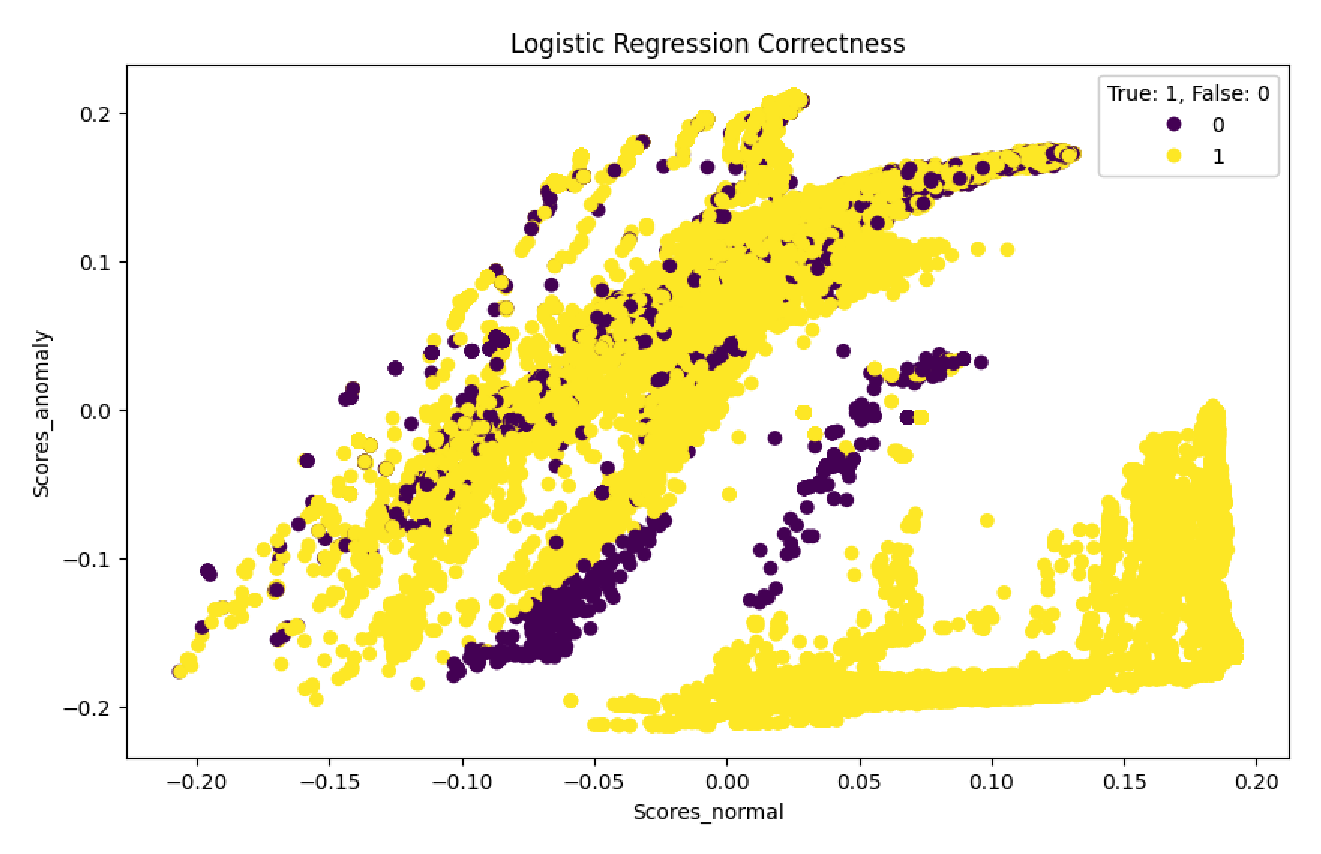
\includegraphics[width=\linewidth]{pictures/eps/collectness_UNSW2.eps}
    \caption{collectness\_UNSW2に関する図の説明(和文)}
    \ecaption{Description of the collectness\_UNSW2 figure (English).}
    \label{fig:collectness_UNSW2}
\end{figure}

\begin{figure}[tb]
    \centering
    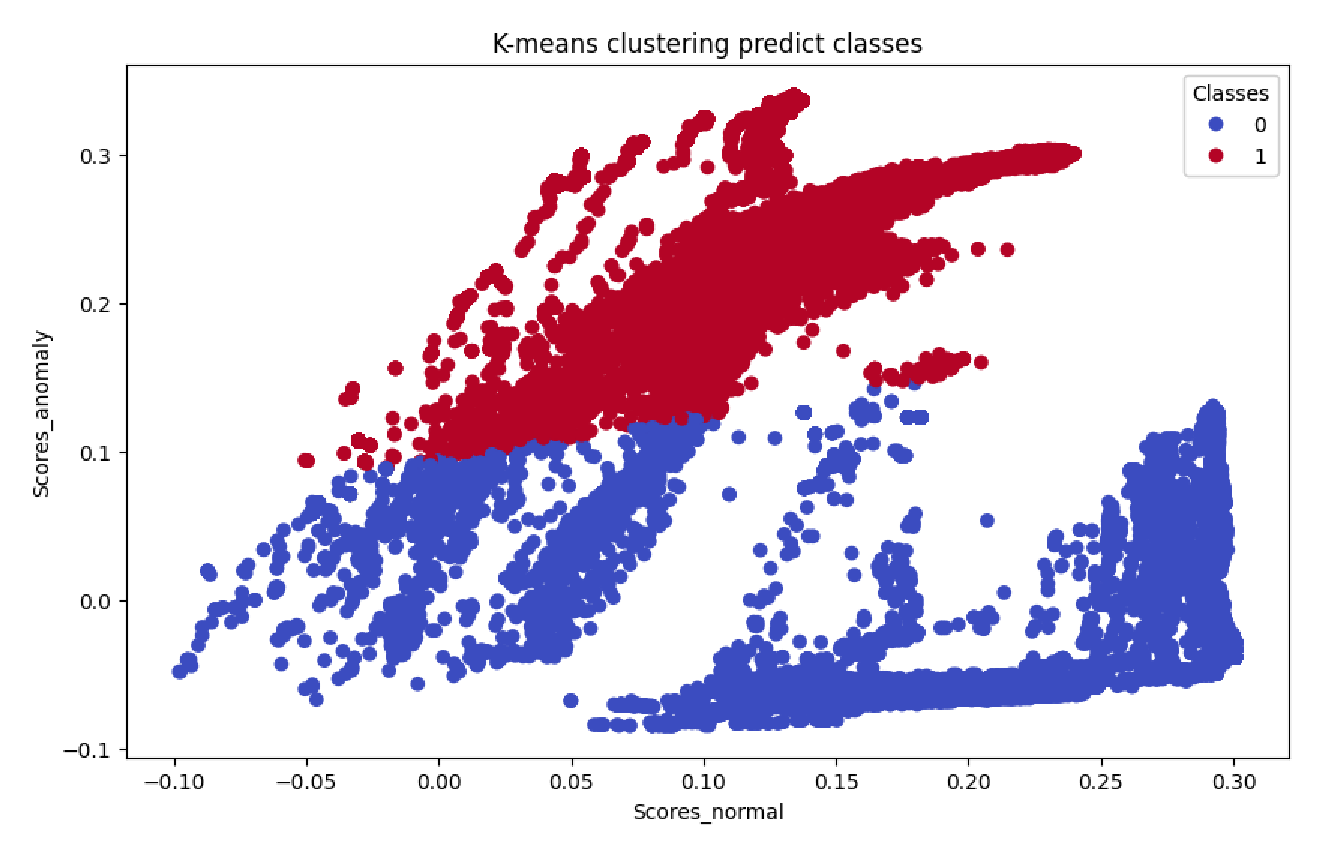
\includegraphics[width=\linewidth]{pictures/eps/predict_classes_UNSW.eps}
    \caption{predict\_classes\_UNSWに関する図の説明(和文)}
    \ecaption{Description of the predict\_classes\_UNSW figure (English).}
    \label{fig:predict_classes_UNSW}
\end{figure}

\begin{figure}[tb]
    \centering
    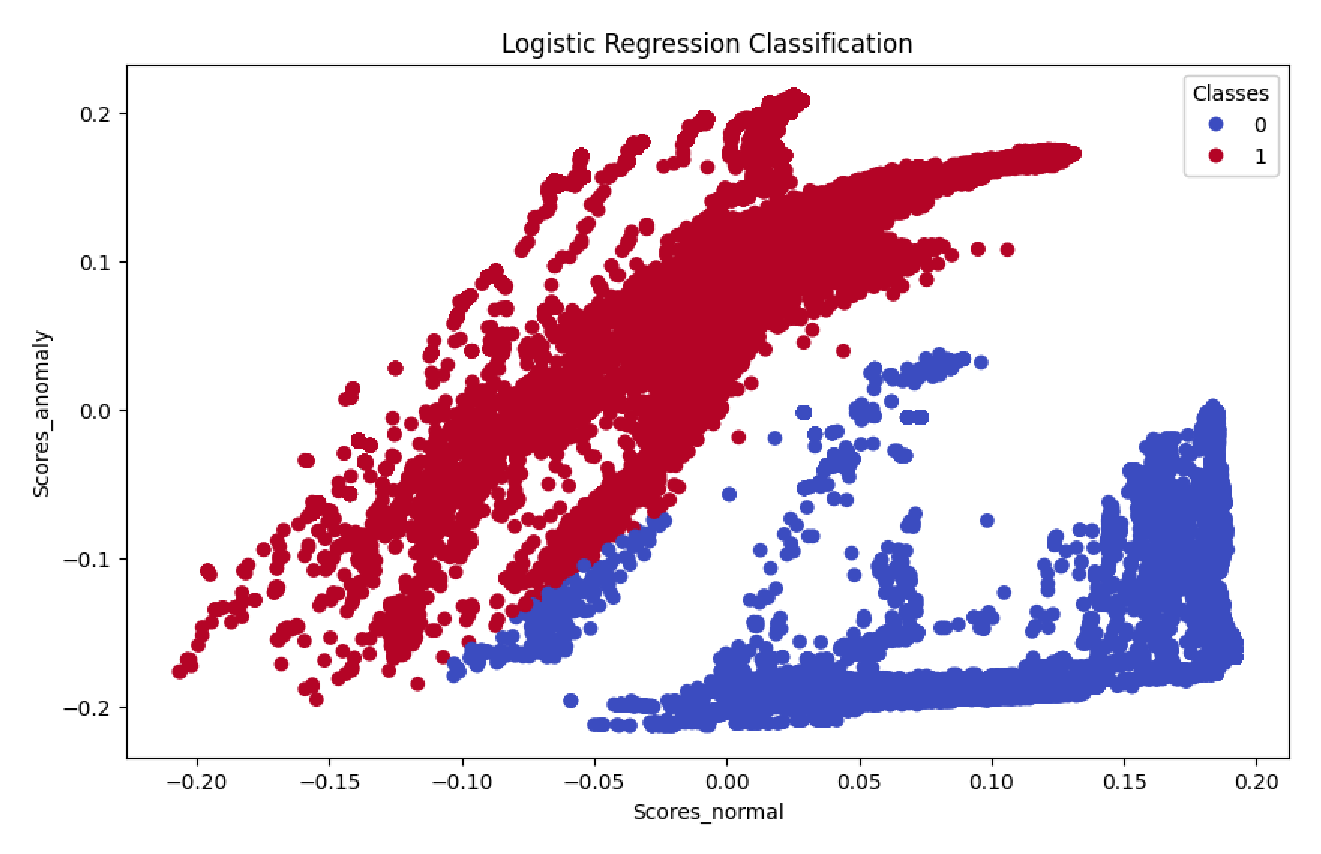
\includegraphics[width=\linewidth]{pictures/eps/predict_classes_UNSW2.eps}
    \caption{predict\_classes\_UNSW2に関する図の説明(和文)}
    \ecaption{Description of the predict\_classes\_UNSW2 figure (English).}
    \label{fig:predict_classes_UNSW2}
\end{figure}

\subsection{考察}

\subsubsection{本論文における目的に即した結論を導く}
\begin{itemize}
    \item 本結果を一般化したどのような結論を導き出せるかを,論文の目的に即して述べる. 1. このくらい有効特徴量あればいける 2.iforestではうまくいく
    \item 実験結果の妥当性を説明する.
\end{itemize}

\subsubsection{結果から予測される問題を提起する.}
\begin{itemize}
    \item 結果が生じた理由について考察する. 1. 2.グラフの分布を見ると、縦横で切るより斜めで切ったほうがいい
    \item 本実験結果を認めると,どのような現象の予測や応用可能性があるかを述べる.1.2.より良い局面、より良いアルゴリズムがあるかも
\end{itemize}

\section{おわりに}
おわりにを書く.

\begin{acknowledgment}
謝辞を書く.
\end{acknowledgment}

\begin{thebibliography}{10}

\end{thebibliography}

\end{document}
